\section{Tìm hiểu về Composite Design Pattern trong OOP.}

\subsection{Khái niệm về Composite Design Pattern.}
Mẫu thiết kế tổng hợp (Composite Design Pattern) là một mẫu thiết kế cấu trúc (Structural Design Pattern) 
mà nó sẽ tổ chức các đối tượng thành cấu trúc cây (trees) để biểu diễn quan hệ toàn thể - bộ phận (whole-part hierarchy).

\subsection{Mục đích của Composite Design Pattern.}
Composite Design Pattern cho phép phía client xử lý các đối tượng riêng lẻ và nhóm đối tượng một cách thống nhất bằng cách sử dụng giao diện chung, 
giúp đơn giản hóa mã nguồn và hỗ trợ mở rộng dễ dàng mà không cần sửa đổi logic ở phía client.

\subsection{Các thành phần của Composite Design Pattern.}
\begin{itemize}
    \item[$-$] \textbf{Component:} giao diện chung cho tất cả đối tượng. 
                Nó định nghĩa các phương thức chung cho cả đối tượng leaf và composite.
    \item[$-$] \textbf{Leaf:} là một đối tượng riêng lẻ, không có đối tượng con. 
                Nó giúp triển khai giao diện thành phần (component) và cung cấp chức năng cụ thể cho các đối tượng riêng lẻ.
    \item[$-$] \textbf{Composite:} là đối tượng chứa, có thể bao gồm các đối tượng lá (leaf) cũng như các đối tượng composite khác. 
                Nó triển khai giao diện thành phần (component) và cung cấp các phương thức để thêm, xóa và truy cập các phần tử con.
    \item[$-$] \textbf{Client:} chịu trách nhiệm sử dụng giao diện thành phần (component) để làm việc với các đối tượng trong cấu trúc. 
                Nó xử lý các đối tượng lá và thành phần một cách thống nhất.
\end{itemize}

\begin{center}
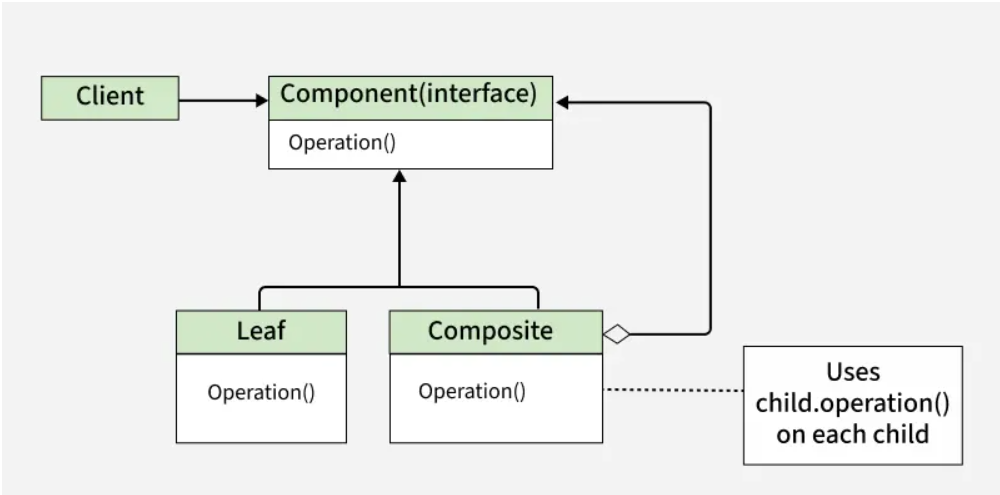
\includegraphics[width=0.75\textwidth]{images/CompositeDesignPattern.png}
\end{center}

-- \textbf{Giải thích:}
\begin{itemize}
    \item[$+$] Phía Client tương tác với giao diện Component, cho phép nó làm việc đồng bộ với tất cả các đối tượng Leaf và Composite.
    \item[$+$] Leaf biểu thị các đối tượng riêng lẻ, trong khi Composite biểu thị một nhóm các đối tượng và có thể chứa nhiều đối tượng con.
    \item[$+$] Lớp Composite gọi đệ quy các phép toán trên các thành phần con của nó và tạo thành cấu trúc dạng cây.
\end{itemize}

\subsection{Phân cấp đối tượng bộ phận-toàn thể (part-whole).}
\textbf{Tác dụng:} Cấu trúc phân cấp này giúp biểu diễn các đối tượng phức tạp (toàn thể) được cấu tạo từ các đối tượng đơn giản hơn (bộ phận).
                   Nó cho phép xử lý đồng nhất cả các đối tượng riêng lẻ và các nhóm đối tượng, thường được mô hình hóa bằng cách sử dụng Composite Design Pattern.

-- \textbf{Ví dụ minh họa:} Một ứng dụng thiết kế đồ họa sẽ có các hình dạng riêng lẻ (hình tròn, chữ nhật,\dots).
Ta có thể kết hợp các hình này để tạo ra các hình dạng phức tạp hơn (ví dụ: hình mặt cười có mắt và miệng).
Composite Design Pattern cho phép ta làm việc với các hình đơn giản và phức tạp bằng cùng một tập hợp các thao tác, 
giúp việc quản lý chúng dễ dàng hơn.

\begin{center}
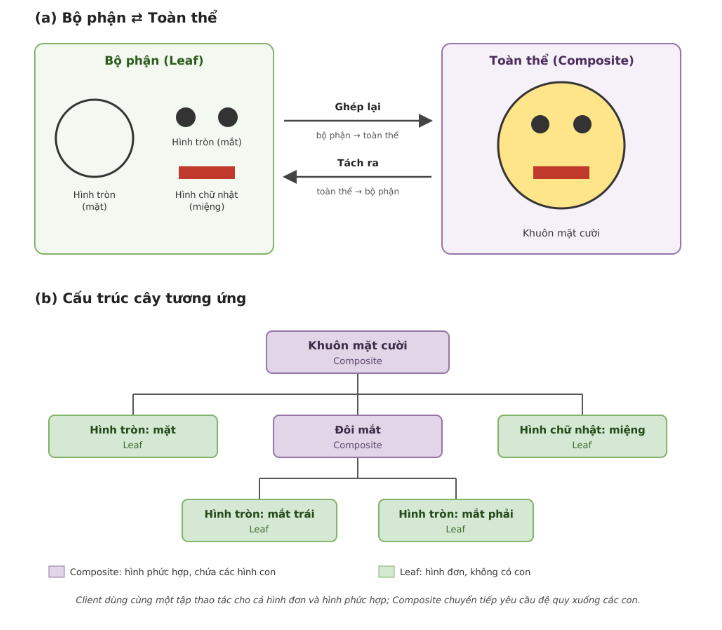
\includegraphics[width=0.85\textwidth]{images/WholePartExample.png}
\end{center}

-- \textbf{Giải thích:}
\begin{itemize}
    \item[$+$] Các bộ phận (parts) là các hình dạng riêng lẻ (hình tròn, hình chữ nhật).
    \item[$+$] Toàn thể (whole) là những hình dạng phức tạp (như hình mặt cười ở trên được tạo thành từ các hình tròn và hình chữ nhật).
\end{itemize}

\subsection{Mã nguồn minh họa cho Composite Design Pattern.}
Ví dụ sau đây minh họa cho biểu thức: $ (2 + 6) * 9 = 72  $.

\lstinputlisting{code/Cau03_Code01.cpp}

-- \textbf{Giải thích:}
\begin{itemize}
    \item[$+$] Hàm main() chính là Client sử dụng Component để làm việc với các đối tượng trong Composite. 
               Trong ví dụ thì chỉ làm việc với nút root.
    \item[$+$] Expression là một Component chung cho tất cả các thành phần trong biểu thức, cả phép nhân, phép cộng, hay là con số.
    \item[$+$] Number là class kế thừa Expression, nó đại diện cho một con số và không sở hữu thêm bất cứ object nào có lớp kế thừa hay là Expression 
               nên nó là Node Leaf trong cấu trúc cây.
    \item[$+$] Multiply và Add là hai class kế thừa Expression và lần lượt đại diện cho hai phép nhân và phép cộng. 
               Trong hai class này, có chứa hai object left and right là hai con trỏ kiểu Expression*. 
               Hai con trỏ left và right có thể là Number, Multiply hay là Add.
    \item[$+$] Luồng chạy: nó sẽ chạy từ root là phép (2 + 6) * 9 trong này left là object Add và right là một object Number. 
               Sau trong evaluate của root thì lại có left->evaluate() thì nó sẽ gọi đệ quy xuống object Add và thực hiện tiếp phép tính cộng gọi left->evaluate() và right->evaluate() của object Add đó. 
               Hết rồi, nó sẽ qua right->evaluate của root và chạy sang object Number lấy con số từ evaluate() của object Number đó.
    \item[$+$] Khi kết thúc, ta gọi delete root thì nó cũng sẽ gọi destructor của các thành phần bên trong nó. 
               Luồng root -> left là biểu thức 2 + 6 -> qua left là số 2 -> qua right là số 6 -> qua right của root là số 9.
\end{itemize}